\begin{frame}[fragile]{And state is stored in a disk (not a memory).}
  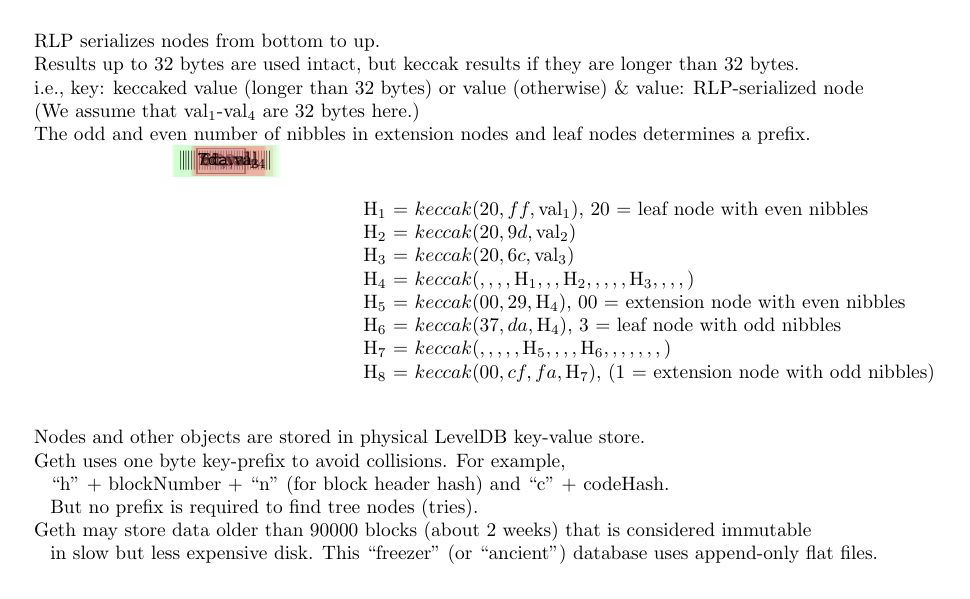
\begin{tikzpicture}[scale=0.7,every node/.style={transform shape}]

\node[align=left,anchor=north west] at (0em,0ex) {
RLP serializes nodes from bottom to up.\\
Results up to 32 bytes are used intact, but keccak results if they are longer than 32 bytes.\\
i.e., key: keccaked value (longer than 32 bytes) or value (otherwise) \& value: RLP-serialized node\\
(We assume that val\textsubscript{1}-val\textsubscript{4} are 32 bytes here.)\\
The odd and even number of nibbles in extension nodes and leaf nodes determines a prefix.};

\begin{scope}[xshift=10em,yshift=-16ex]
\tikzstyle{treenode}=[fill opacity=0.2,text opacity=1]
\tikzset{edge from parent/.style={draw,edge from parent path={(\tikzparentnode.south) -- +(0,-0.6ex) -| (\tikzchildnode.north)}}}
\Tree [ .\node[draw]{root};
  \edge node[auto=right]{\footnotesize{H\textsubscript{8}}}; [ .\node[treenode,fill=blue!50]{\texttt{c7fa}};
    \edge node[auto=right]{\footnotesize{H\textsubscript{7}}}; [ .\node[treenode,fill=green!50]{$|||||||||||||||||$};
      \edge node[auto=right]{\footnotesize{5 H\textsubscript{5}}}; [ .\node[treenode,fill=blue!50]{\texttt{29}};
        \edge node[auto=right]{\footnotesize{H\textsubscript{4}}}; [ .\node[treenode,fill=green!50]{$|||||||||||||||||$};
          \edge node[auto=right]{\footnotesize{4 H\textsubscript{1}}}; \node[treenode,fill=red!50]{\texttt{ff},val\textsubscript{1}};
          \edge node[auto=right]{\footnotesize{7 H\textsubscript{2}}}; \node[treenode,fill=red!50]{\texttt{9d},val\textsubscript{2}};
          \edge node[auto=left]{\footnotesize{c H\textsubscript{3}}}; \node[treenode,fill=red!50]{\texttt{6c},val\textsubscript{3}};
        ]
      ]
      \edge node[auto=left]{\footnotesize{9 H\textsubscript{6}}}; \node[treenode,fill=red!50]{\texttt{7da},val\textsubscript{4}};
  ]
]]
\end{scope}

\node[align=left,anchor=north west] at (17em,-20ex) {
H\textsubscript{1} = $keccak(20,ff,\textnormal{val\textsubscript{1}})$, 20 = leaf node with even nibbles\\
H\textsubscript{2} = $keccak(20,9d,\textnormal{val\textsubscript{2}})$\\
H\textsubscript{3} = $keccak(20,6c,\textnormal{val\textsubscript{3}})$\\
H\textsubscript{4} = $keccak(\varnothing,\varnothing,\varnothing,\varnothing,\textnormal{H\textsubscript{1}},\varnothing,\varnothing,\textnormal{H\textsubscript{2}},\varnothing,\varnothing,\varnothing,\varnothing,\textnormal{H\textsubscript{3}},\varnothing,\varnothing,\varnothing,\varnothing)$\\
H\textsubscript{5} = $keccak(00,29,\textnormal{H\textsubscript{4}})$, 00 = extension node with even nibbles\\
H\textsubscript{6} = $keccak(37,da,\textnormal{H\textsubscript{4}})$, 3$\square$ = leaf node with odd nibbles\\
H\textsubscript{7} = $keccak(\varnothing,\varnothing,\varnothing,\varnothing,\varnothing,\textnormal{H\textsubscript{5}},\varnothing,\varnothing,\varnothing,\textnormal{H\textsubscript{6}},\varnothing,\varnothing,\varnothing,\varnothing,\varnothing,\varnothing,\varnothing)$\\
H\textsubscript{8} = $keccak(00,cf,fa,\textnormal{H\textsubscript{7}})$, (1$\square$ = extension node with odd nibbles)
};

\node[align=left,anchor=north west] at (0em,-47.5ex) {
Nodes and other objects are stored in physical LevelDB key-value store.\\
Geth uses one byte key-prefix to avoid collisions. For example,\\
\hspace{0.5em} ``h'' + blockNumber + ``n'' (for block header hash) and ``c'' + codeHash.\\
\hspace{0.5em} But no prefix is required to find tree nodes (tries).\\
Geth may store data older than 90000 blocks (about 2 weeks) that is considered immutable\\
\hspace{0.5em} in slow but less expensive disk. This ``freezer'' (or ``ancient'') database uses append-only flat files.
};

  \end{tikzpicture}
\end{frame}